\documentclass{article}

% Language setting
% Replace `english' with e.g. `spanish' to change the document language
\usepackage[utf8]{inputenc}
\usepackage{polski}

% Set page size and margins
% Replace `letterpaper' with `a4paper' for UK/EU standard size
\usepackage[letterpaper,top=2cm,bottom=2cm,left=3cm,right=3cm,marginparwidth=1.75cm]{geometry}

\usepackage{float}

% Useful packages
\usepackage{amsmath}
\usepackage{graphicx}
\usepackage[colorlinks=true, allcolors=blue]{hyperref}

\title{Baza danych medium społecznościowego}
\author{Łukasz Fabia 272724 \\ Mikołaj Kubś ... \\ Projektowanie baz danych wt 18:55}

\begin{document}
\maketitle

\tableofcontents

\section{Etap 1: Faza konceptualna}

\subsection{Analiza świata rzeczywistego}

\subsubsection{Streszczenie - Zarys wymagań projektu}

Celem projektu jest stworzenie bazy danych do obsługi medium społecznościowego. Ma ona przechowywać informacje o użytkownikach, ich treściach, relacjach i aktywnościach. Baza powinna być zaprojektowana w sposób wydajny i skalowalny.

\subsubsection{Potrzeby informacyjne}
\begin{itemize}
    \item Rejestracja i logowanie użytkowników z różnymi poziomami dostępu.
    \item Publikowanie i interakcje z treściami użytkowników (posty, polubienia, komentarze).
    \item Zarządzanie relacjami społecznymi (znajomości).
    \item Przechowywanie wiadomości prywatnych i historii aktywności.
    \item Tworzenie konwersacji z innymi użytkownikami
    \item Reportowanie postów z nieodpowiednimi treśćmi
    \item Tworzenie i zarządzanie stronami organizacji, firm, fanpage itd.
    \item Tworzenie i zarządzanie wydarzeniami
\end{itemize}

\subsubsection{Czynności, wyszukiwania}

\begin{itemize}
    \item Wyszukiwanie użytkowników.
    \item Wyszukiwanie treści po hasztagach lub słowach kluczowych.
    \item Filtrowanie aktywności użytkownika, np. przeglądanie polubień i komentarzy.
    \item Wyszukiwanie relacji (np. znajomi użytkownika, osoby obserwujące daną osobę).
    \item Dodawanie innych użytkowników do znajomych i interakcja z treściami - dodawanie komentarzy i reakcji
    \item Tworzenie postów, wydarzeń, grup
    \item Konwersacja grupowa, pisanie wiadomości
\end{itemize}

\subsubsection{Cele projektu}

\begin{tabular}{@{} l p{12cm} @{}}
    \textbf{S (Specific)}: & Zaprojektowanie bazy danych dla medium społecznościowego. \\ \\
    \textbf{M (Measurable)}: & Baza musi być wydajna, tzn. musi być w stanie obsługiwać dużą ilość użytkowników, co najmniej 20 000. \\ \\
    \textbf{A (Achievable)}: & Projekt zostanie zrealizowany przy użyciu PostgreSQL. Do stworzenia struktury tabel wykorzystany zostanie mechanizm ORM (Object Relational Mapping). Na koniec baza zostanie wypełniona danymi, aby przetestować jej wydajność. \\ \\
    \textbf{R (Relevant)}: & Przechowywanie profili użytkowników oraz interakcje między nimi są kluczowe dla funkcjonowania medium społecznościowego. \\ \\
    \textbf{T (Time-bound)}: & Praca nad projektem powinna zająć 2 miesiące.
\end{tabular}

\subsubsection{Zakres projektu}

\begin{tabular}{@{} l p{10cm} @{}}
    \textbf{Multimedia}: & W bazie przechowywane będą wyłącznie linki do plików na zewnętrznym serwerze. \\
    \textbf{Obsługa haseł}: & Wszystkie hasła w bazie będą hashowane.
\end{tabular}


\subsection{Wymagania funkcjonalne}

\begin{abstract}
    Użytkownikom przypisany jest jeden z tych poziomów dostępu: admin, user lub guest.
\end{abstract}

\textbf{Guest(Gość)}

\begin{itemize}
    \item Może przeglądać wybrane dane.
\end{itemize}

\textbf{Admin}

\begin{itemize}
    \item Może przeglądać, edytować, usuwać, dodawać i przeglądać wszystkie treści, zrządza bazą i nadaje uprawnienia
\end{itemize}

\textbf{User(Użytkownik)}

\begin{itemize}
    \item System umożliwia rejestrację oraz logowanie.
    \item Rejestracja wymaga imienia, nazwiska, daty urodzenia, hasła oraz maila.
    \item Logowanie wymaga maila i hasła.
\end{itemize}


\subsection{ERD}

\begin{figure}[H]
    \centering
    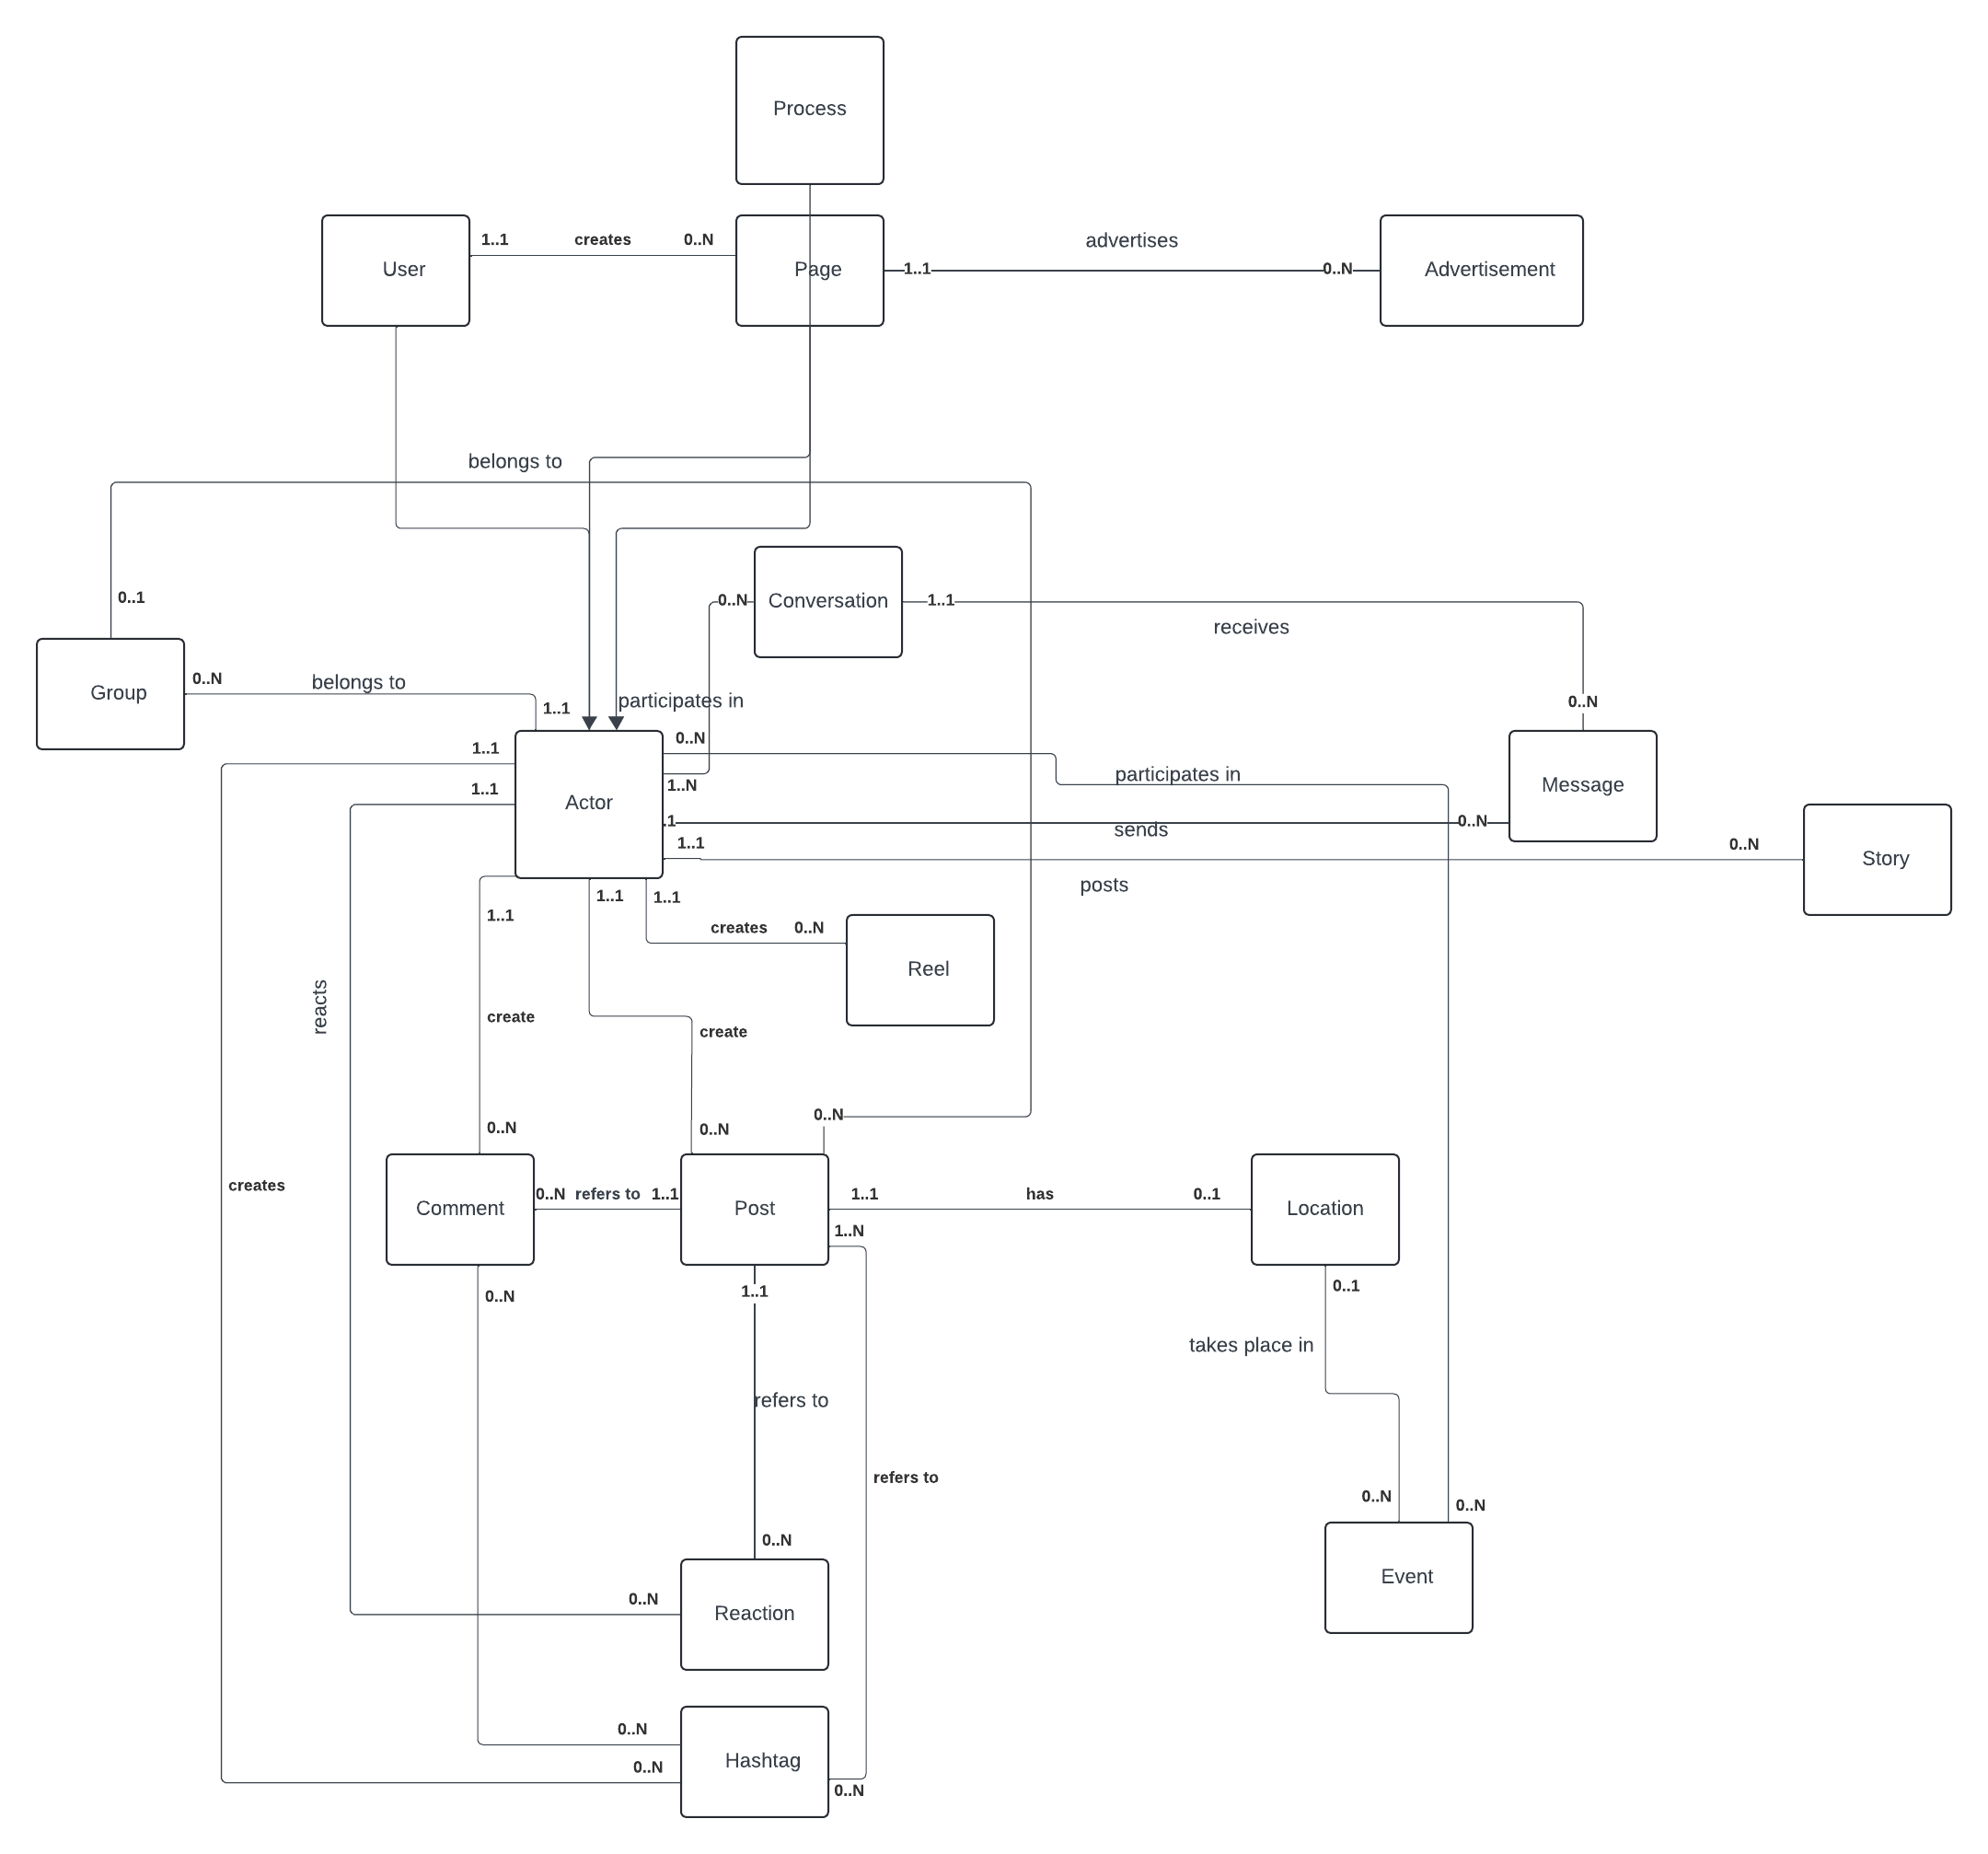
\includegraphics[width=\linewidth]{images/Blank diagram.png}
    \caption{Diagram obiektowo-relacyjny}
    \label{fig:erd}
\end{figure}

\end{document}